% DPF 09 talk on strangeness in nucleon

\documentclass[10pt]{beamer}
\usepackage{amsmath}
\usepackage{mathtools}
\usefonttheme{professionalfonts} % using non standard fonts for beamer
\usefonttheme{serif} % default family is serif
%\documentclass[12pt]{beamerthemeSam.sty}
\usepackage{epsf}
%\usepackage{pstricks}
%\usepackage[orientation=portrait,size=A4]{beamerposter}
\geometry{paperwidth=160mm,paperheight=120mm}
%DT favorite definitions
\def\LL{\left\langle}	% left angle bracket
\def\RR{\right\rangle}	% right angle bracket
\def\LP{\left(}		% left parenthesis
\def\RP{\right)}	% right parenthesis
\def\LB{\left\{}	% left curly bracket
\def\RB{\right\}}	% right curly bracket
\def\PAR#1#2{ {{\partial #1}\over{\partial #2}} }
\def\PARTWO#1#2{ {{\partial^2 #1}\over{\partial #2}^2} }
\def\PARTWOMIX#1#2#3{ {{\partial^2 #1}\over{\partial #2 \partial #3}} }

\def\rightpartial{{\overrightarrow\partial}}
\def\leftpartial{{\overleftarrow\partial}}
\def\diffpartial{\buildrel\leftrightarrow\over\partial}

\def\BI{\begin{itemize}}
\def\EI{\end{itemize}}
\def\BE{\begin{displaymath}}
\def\EE{\end{displaymath}}
\def\BEA{\begin{eqnarray*}}
\def\EEA{\end{eqnarray*}}
\def\BNEA{\begin{eqnarray}}
\def\ENEA{\end{eqnarray}}
\def\EL{\nonumber\\}


\newcommand{\etal}{{\it et al.}}
\newcommand{\gbeta}{6/g^2}
\newcommand{\la}[1]{\label{#1}}
\newcommand{\ie}{{\em i.e.\ }}
\newcommand{\eg}{{\em e.\,g.\ }}
\newcommand{\cf}{cf.\ }
\newcommand{\etc}{etc.\ }
\newcommand{\atantwo}{{\rm atan2}}
\newcommand{\Tr}{{\rm Tr}}
\newcommand{\dt}{\Delta t}
\newcommand{\op}{{\cal O}}
\newcommand{\msbar}{{\overline{\rm MS}}}
\def\chpt{\raise0.4ex\hbox{$\chi$}PT}
\def\schpt{S\raise0.4ex\hbox{$\chi$}PT}
\def\MeV{{\rm Me\!V}}
\def\GeV{{\rm Ge\!V}}

%AB: my color definitions
%\definecolor{mygarnet}{rgb}{0.445,0.184,0.215}
%\definecolor{mygold}{rgb}{0.848,0.848,0.098}
%\definecolor{myg2g}{rgb}{0.647,0.316,0.157}
\definecolor{abtitlecolor}{rgb}{0.0,0.255,0.494}
\definecolor{absecondarycolor}{rgb}{0.0,0.416,0.804}
\definecolor{abprimarycolor}{rgb}{1.0,0.686,0.0}
\definecolor{Red}           {cmyk}{0,1,1,0}
\definecolor{Grey}           {cmyk}{.7,.7,.7,0}
\definecolor{Blue}          {cmyk}{1,1,0,0}
\definecolor{Green}         {cmyk}{1,0,1,0}
\definecolor{Brown}         {cmyk}{0,0.81,1,0.60}

\usetheme{Madrid}


%AB: redefinition of beamer colors
%\setbeamercolor{palette tertiary}{fg=white,bg=mygarnet}
%\setbeamercolor{palette secondary}{fg=white,bg=myg2g}
%\setbeamercolor{palette primary}{fg=black,bg=mygold}
\setbeamercolor{title}{fg=abtitlecolor}
\setbeamercolor{frametitle}{fg=abtitlecolor}
\setbeamercolor{palette tertiary}{fg=white,bg=abtitlecolor}
\setbeamercolor{palette secondary}{fg=white,bg=absecondarycolor}
\setbeamercolor{palette primary}{fg=black,bg=abprimarycolor}
\setbeamercolor{structure}{fg=abtitlecolor}

\setbeamerfont{section in toc}{series=\bfseries}

%AB: remove navigation icons
\beamertemplatenavigationsymbolsempty
\title[1D kinematics]{
  \textbf {1D kinematics: solving problems} 
%\centerline{}
%\centering
%\vspace{-0.0in}
%\includegraphics[width=0.3\textwidth]{propvalues_0093.pdf}
%\vspace{-0.3in}\\
%\label{intrograph}
}

\author[W. Freeman] {Physics 211\\Syracuse University, Physics 211 Spring 2016\\Walter Freeman}

\date{\today}

\begin{document}

\frame{\titlepage}

\frame{\frametitle{\textbf{On solving problems}}
\large
\begin{center}
\color{Red}
You can recognize truth by its beauty and simplicity. 
When you get it right, it is obvious that it is right--at least if you have any experience--because 
usually what happens is that more comes out than goes in....
{[}i{]}nexperienced students make guesses that are very complicated, {[}but{]} the truth always turns out to be simpler than you thought.

\bigskip

\end{center}
\bigskip
--Richard Feynman, quoted by K. C. Cole, in {\it Sympathetic Vibrations: Reflections on Physics as a Way of Life (1985)}

\bigskip
\bigskip
\bigskip
\bigskip

\begin{center}
\color{Red}
Nature uses only the longest threads to weave her patterns, so each small piece of her fabric reveals the organization of the entire tapestry.
\bigskip

\end{center}
\bigskip
--Richard Feynman, {\it The Character of Physical Law} (1965) 



}



\frame{\frametitle{\textbf{Announcements}}
\large
\BI
\item{Homework 1 due tomorrow -- note the Homework Guidebook link on the website}
\item{Clickers introduced in class today}
\item{I'm seeing lots of you in the Clinic; I'd like to see lots more}
\item{{\bf Extended clinic hours:} today from 3:30-6:30 and perhaps from 1:15-2}
\item{I'm hiring extra coaches to work in the Clinic tomorrow afternoon}
\EI
}

\frame{\frametitle{\textbf{Announcements}}

\Large

Did someone lose a piece of jewelry? Tell me if you did...

}
\frame{\frametitle{\textbf{Clicker registration}}
\large
\BI
\item{We're starting clicker questions today in class}
\item{This is a new thing for me -- it's a learning experience for us both!}
\item{Clicker registration instructions on the course website}
\item{You don't need to register until next week}
\EI
}

\bigskip



\frame{\frametitle{\textbf{``Ask a Physicist''}}
\Large

Submit questions!

}

\frame{\frametitle{\textbf{Today}}
\Large
\BI
\item{Clicker introduction}
\item{Review material from last time}
\item{Rotational kinematics}
\item{Concepts for problem solving}
\item{The ``2x2 framework''}
\item{Sample problems}
\pause
\item{Homework help?}
\EI
}

\frame{\frametitle{\textbf{Poll questions}}
\Large
How are you answering this question?

\BI
\item{A. A clicker}
\item{B. A smartphone}
\item{C. Semaphore flags}
\EI
}

\frame{\frametitle{\textbf{Poll questions}}
\Large
What's your experience with spreadsheet software?

\BI
\item{A. None}
\item{B. I'm familiar with Google Sheets/Docs}
\item{C. I'm familiar with Excel or LibreOffice, but not Google Sheets}
\item{D. I've never used a spreadsheet, but know C/Python/Java/Pascal/etc.}
\EI
}

\frame{\frametitle{\textbf{Poll questions}}
\Large
What sort of computing hardware do you have, or could you borrow, for recitation periods next week?

\BI
\item{A. A laptop (including Chromebooks, netbooks, etc.}
\item{B. A tablet (iPad, etc.)}
\item{C. Neither (don't worry; we'll take care of you!)}
\EI
}

\frame{\frametitle{\textbf{Poll questions}}
\Large
What's your experience studying physics?

\BI
\item{A. None (that's okay!)} 
\item{B. A university/college physics course}
\item{C. An AP or International Baccalaureate high school physics course}
\item{D. Another high school physics course}
\EI
}


\frame{\frametitle{\textbf{Last time: Position, velocity, and acceleration}}
\begin{columns}
\column{0.125\textwidth}
\centerline{\Large Position}
\column{0.2\textwidth}
\small
{\color{Red}
\centerline{(derivative of)}
\centerline{rate of change of}
\centerline{$\xleftarrow{\makebox[\textwidth]{}}$}}
{\color{Green}
\color{Green}\centerline{$\xrightarrow{\makebox[\textwidth]{}}$}}
\color{Green}\centerline{area under the curve of}
\color{Green}\centerline{(integral of)}
\column{0.125\textwidth}
\centerline{\Large Velocity}
\pause
\column{0.2\textwidth}
\small
{\color{Red}
\centerline{(derivative of)}
\centerline{rate of change of}
\centerline{$\xleftarrow{\makebox[\textwidth]{}}$}}
{\color{Green}
\color{Green}\centerline{$\xrightarrow{\makebox[\textwidth]{}}$}}
\color{Green}\centerline{area under the curve of}
\color{Green}\centerline{(integral of)}
\column{0.15\textwidth}
\centerline{\Large Acceleration}
\end{columns}
}



\frame{\frametitle{\textbf{Position, velocity, and acceleration}}
\begin{columns}
\column{0.125\textwidth}
\centerline{\Large Position}
\column{0.2\textwidth}
\small
{\color{Red}
\centerline{(derivative of)}
\centerline{rate of change of}
\centerline{$\xleftarrow{\makebox[\textwidth]{}}$}}
\column{0.125\textwidth}
\centerline{\Large Velocity}
\pause
\column{0.2\textwidth}
\small
{\color{Red}
\centerline{(derivative of)}
\centerline{rate of change of}
\centerline{$\xleftarrow{\makebox[\textwidth]{}}$}}
\column{0.15\textwidth}
\centerline{\Large Acceleration}
\end{columns}
}

\frame{\frametitle{\textbf{Kinematics}}
\Large
\BI
\item{If we know acceleration as a function of time, how do we get from there to position vs. time?}
\pause

\bigskip
\bigskip
\bigskip
\item{A. Look at the slope of the acceleration vs. time graph to get velocity, and then look at its slope to get position}
\item{B. Look at the area under the curve of the acceleration vs. time graph to get velocity, and then look at the area under {\it} that graph to get position}
\item{C. Take two derivatives of the acceleration vs. time graph to get position vs. time}
\item{D. Take two integrals of the acceleration vs. time graph to get position vs. time}
\EI
}

\frame{\frametitle{\textbf{The ``kinematics equations''}}

{\color{Red}
\Large
\begin{align*}
v(t) =& at + v_0 \\
x(t) =& \frac{1}{2}at^2 + v_0 t + x_0
\end{align*}}

\bigskip
\bigskip
\bigskip

These equations are valid when...
\BI
\item{A. Acceleration is constant}
\item{B. Velocity is constant}
\item{C. The object moves in only one direction}
\item{D. They are always valid}
\pause
\bigskip
\bigskip
\item{A: these are the expressions for $x(t)$ and $v(t)$ when acceleration is constant!}
\EI
}

\frame{\frametitle{\textbf{Rotational kinematics}}
\Large
\BI
\item{Linear motion: care about position as a function of time}
\item{Rotational motion: care about {\color{Red}angle} as a function of time}
\item{\bf Everything we just did translates to rotational kinematics exactly!}
\EI
}

\frame{\frametitle{\textbf{Position, velocity, and acceleration}}
\begin{columns}
\column{0.125\textwidth}
\centerline{\Large Position}
\column{0.2\textwidth}
\small
{\color{Red}
\centerline{(derivative of)}
\centerline{rate of change of}
\centerline{$\xleftarrow{\makebox[\textwidth]{}}$}}
{\color{Green}
\color{Green}\centerline{$\xrightarrow{\makebox[\textwidth]{}}$}}
\color{Green}\centerline{area under the curve of}
\color{Green}\centerline{(integral of)}
\column{0.125\textwidth}
\centerline{\Large Velocity}
\pause
\column{0.2\textwidth}
\small
{\color{Red}
\centerline{(derivative of)}
\centerline{rate of change of}
\centerline{$\xleftarrow{\makebox[\textwidth]{}}$}}
{\color{Green}
\color{Green}\centerline{$\xrightarrow{\makebox[\textwidth]{}}$}}
\color{Green}\centerline{area under the curve of}
\color{Green}\centerline{(integral of)}
\column{0.15\textwidth}
\centerline{\Large Acceleration}
\end{columns}
}

\frame{\frametitle{\textbf{Angle, angular velocity, and angular acceleration}}
\begin{columns}
\column{0.125\textwidth}
\centerline{\Large Angle}
\column{0.2\textwidth}
\small
{\color{Red}
\centerline{(derivative of)}
\centerline{rate of change of}
\centerline{$\xleftarrow{\makebox[\textwidth]{}}$}}
{\color{Green}
\color{Green}\centerline{$\xrightarrow{\makebox[\textwidth]{}}$}}
\color{Green}\centerline{area under the curve of}
\color{Green}\centerline{(integral of)}
\column{0.125\textwidth}
\begin{center}
\Large Angular velocity ($\omega$)
\end{center}
\pause
\column{0.2\textwidth}
\small
{\color{Red}
\centerline{(derivative of)}
\centerline{rate of change of}
\centerline{$\xleftarrow{\makebox[\textwidth]{}}$}}
{\color{Green}
\color{Green}\centerline{$\xrightarrow{\makebox[\textwidth]{}}$}}
\color{Green}\centerline{area under the curve of}
\color{Green}\centerline{(integral of)}
\column{0.15\textwidth}
\begin{center}
\large Angular acceleration ($\alpha$)
\end{center}
\end{columns}

\Large
\bigskip
\bigskip
\bigskip

\pause

$$ x(t) = x_0 + v_0 t + \frac{1}{2}at^2 $$

$$ \theta(t) = \theta_0 + \omega_0 t + \frac{1}{2}\alpha t^2 $$

\pause

\bigskip

$\rightarrow$ Angular kinematics works in exactly the same way as translational kinematics!

}

\frame{\frametitle{\textbf{Angle, angular velocity, and angular acceleration}}
\large
\BI
\item{Angle $\theta$ -- the angle through which something has turned.}
\item{Measured in revolutions, radians, degrees...}
\bigskip
\bigskip
\bigskip
\item{Angular velocity $\omega$ (``omega'', not ``dubya'') -- the rate at which something is turning} 
\item{Measured in revolutions per second, radians per second, degrees per second...}
\bigskip
\bigskip
\bigskip
\item{Angular acceleration $\alpha$ (``alpha'', not ``fish'') -- the rate at which something's rate of turning is changing} 
\item{Measured in $\frac{\rm rev}{\rm s^2}$, $\frac{\rm rad}{\rm s^2}$, $\frac{\rm deg}{\rm s^2}$...}
\EI
}

\frame{\frametitle{\textbf{The 2x2 square for organizing your ideas}}
\begin{center}
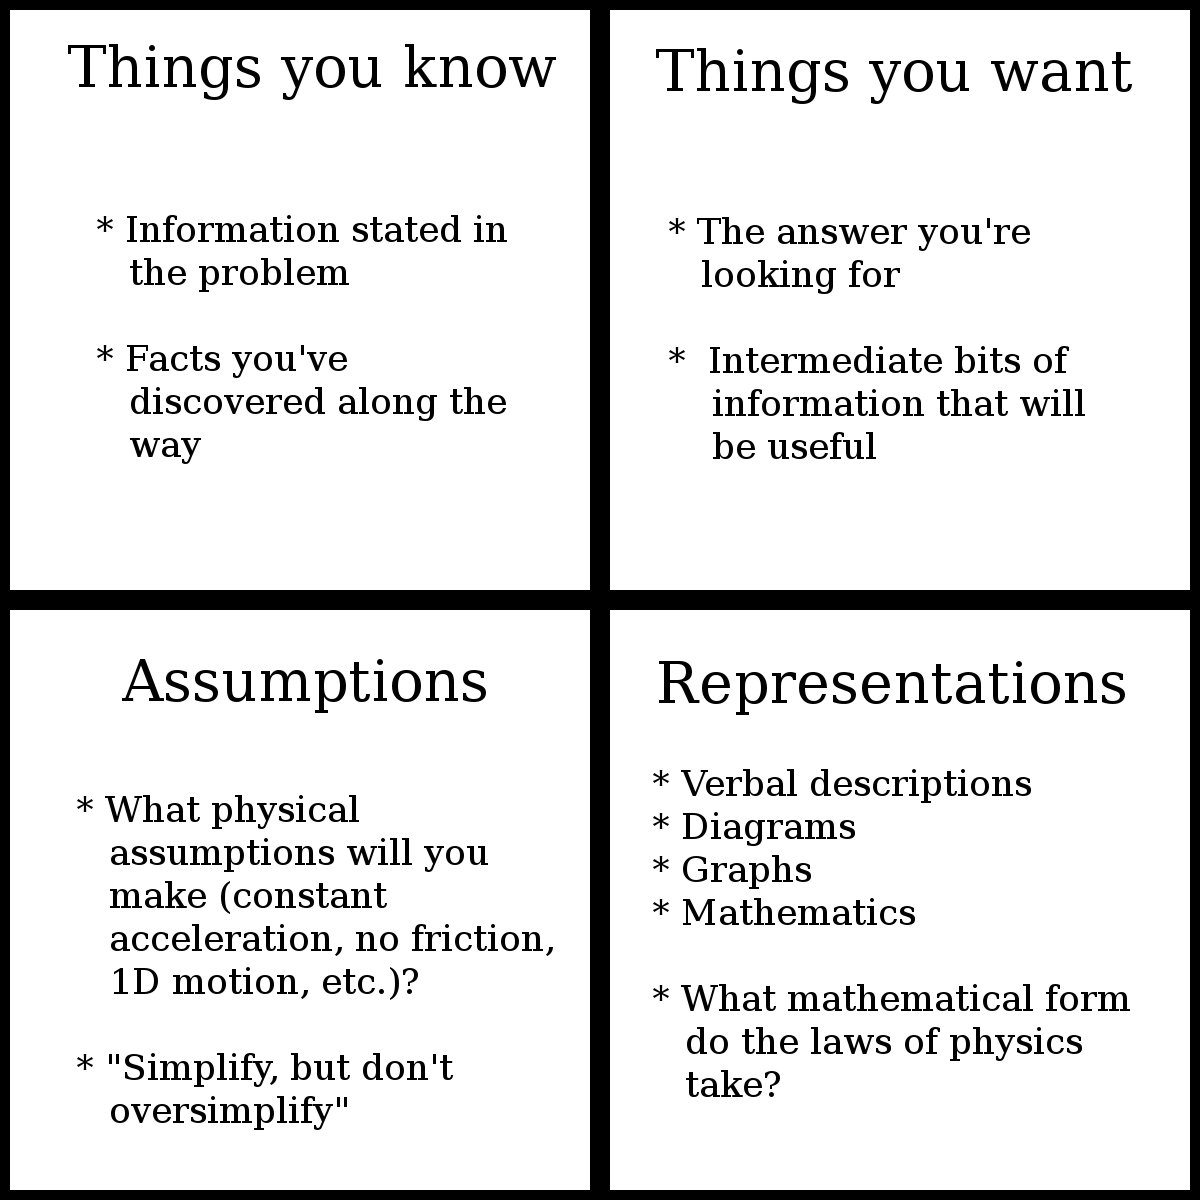
\includegraphics[width=0.5\textwidth]{grid.png}
\end{center}

An excellent tool for you to use when you don't know quite how to proceed...
}


\frame{\frametitle{\textbf{Example problems}}
\Large
\BI
\item{How long does it take for a falling object to fall a height $h$?}
\pause
\bigskip
\bigskip
\bigskip
\item{A. $\sqrt{2g/h}$}
\item{B. $h/g$}
\item{C. $\sqrt{2h/g}$}
\item{D. $2h/g$}
\EI
}

\frame{\frametitle{\textbf{Example problems}}
\Large
\BI
\item{A wheel at rest starts accelerating with an angular acceleration $\alpha$ rad/s. How long does it take to rotate once?}
\EI

\pause

\bigskip
\bigskip
\bigskip

This is the same as the last problem, really!
}


\frame{\frametitle{\textbf{Example problems}}
\Large
\BI
\item{You throw an object up with an initial speed of $5\, \rm m/\rm s$. How high does it go? How long does it take to come back down?}
\EI
}

\frame{\frametitle{\textbf{Example problems}}
\Large
\BI
\item{You throw a ball straight up with an initial speed of $v_1$. A car is moving horizontally at constant speed $v_2$. How far does the car
move before the ball comes back down?}

\EI
}




\frame{\frametitle{\textbf{Another example}}
\Large 
You throw an object up with an initial speed of $v_0$. How long does it take to reach a height $h$?

\pause

\bigskip

\begin{align*}
x(t) = &\hspace{1.25em}\frac{1}{2}at^2 + v_0 t + x_0 \\
h =& -\frac{1}{2}gt^2 + v_0 t \\
0 =& -\frac{1}{2}gt^2 + v_0 t - h
\end{align*}

\large
\BI
\item{$\rightarrow$ {\color{Red}You need the quadratic formula for this -- nonzero $a$, $v_0$, and position}}
\item{The quadratic formula gives you two answers, but there's clearly only one}
\item{The homework asks you to address this idea.}
\item{Hint: graph position vs. time, and interpret the question graphically}
\item{What is the {\it mathematical} interpretation of the quadratic formula?}
\EI
}


\frame{\frametitle{\textbf{Example problems}}
\Large
\BI
\item{A bucket is being lowered from a cliff at a rate of 10 m/s. You drop a rock off the cliff when the bucket is 10 m beneath the top. 
How long does it take for the rock to land in the bucket?}
\EI
}


\end{document}

